\documentclass[]{article}

% Imported Packages
%------------------------------------------------------------------------------
\usepackage{amssymb}
\usepackage{amstext}
\usepackage{amsthm}
\usepackage{amsmath}
\usepackage{enumerate}
\usepackage{fancyhdr}
\usepackage[margin=1in]{geometry}
\usepackage{graphicx}
%\usepackage{extarrows}
%\usepackage{setspace}
%------------------------------------------------------------------------------

% Header and Footer
%------------------------------------------------------------------------------
\pagestyle{plain}  
\renewcommand\headrulewidth{0.4pt}                                      
\renewcommand\footrulewidth{0.4pt}                                    
%------------------------------------------------------------------------------

% Title Details
%------------------------------------------------------------------------------
\title{Deliverable \#2}
\author{SE 3A04: Software Design II -- Large System Design}
\date{}                               
%------------------------------------------------------------------------------

% Document
%------------------------------------------------------------------------------
\begin{document}

\maketitle	
\noindent{\bf Tutorial Number:} T03\\
{\bf Group Number:} G8 \\
{\bf Group Members:} 
\begin{itemize}
	\item Hashim Bukhtiar
	\item Jaden Moore
	\item James Ariache
	\item Olivia Reich
	\item Omar Abdelhamid
\end{itemize}

\section*{IMPORTANT NOTES}
\begin{itemize}
	%	\item You do \underline{NOT} need to provide a text explanation of each diagram; the diagram should speak for itself
	\item Please document any non-standard notations that you may have used
	\begin{itemize}
		\item \emph{Rule of Thumb}: if you feel there is any doubt surrounding the meaning of your notations, document them
	\end{itemize}
	\item Some diagrams may be difficult to fit into one page
	\begin{itemize}
		\item Ensure that the text is readable when printed, or when viewed at 100\% on a regular laptop-sized screen.
		\item If you need to break a diagram onto multiple pages, please adopt a system of doing so and thoroughly explain how it can be reconnected from one page to the next; if you are unsure about this, please ask about it
	\end{itemize}
	\item Please submit the latest version of Deliverable 1 with Deliverable 2
	\begin{itemize}
		\item Indicate any changes you made.
	\end{itemize}
	\item If you do \underline{NOT} have a Division of Labour sheet, your deliverable will \underline{NOT} be marked
\end{itemize}

\newpage
\section{Introduction}
\label{sec:introduction}
% Begin Section

\subsection{Purpose}
\label{sub:purpose}
% Begin SubSection
This document provides a high-level overview of the RideRecon car identification system architecture, including high-level design considerations of the system and design consideration for various subsystems. This document is intended for internal RideRecon stakeholders, including but not limited to, project managers, developers, domain experts, and RideRecon team members/investors. \\

\noindent Note that RideRecon Deliverable 1 should be read before Deliverable 2, and technical knowledge may be beneficial in better understanding this document's contents.

% End SubSection

\subsection{System Description}
\label{sub:system_description}
% Begin SubSection
The RideRecon system is designed to identify vehicles based on both text and image inputs, leveraging multiple expert modules (such as a reverse image search engine, a text-based LLM, and trained ML models). To integrate these diverse experts effectively, RideRecon follows a blackboard architecture. In this approach, all relevant data—user inputs, partial identifications, and expert findings—are posted to a central “blackboard.” Each expert module reads from this shared repository, processes the data according to its specialization, and writes back its results. This iterative process continues until a consensus or a conflict resolution mechanism determines the final identification outcome.\\

\noindent A blackboard architecture is well-suited to RideRecon because it supports concurrent data processing among the different expert modules, each of which may require varying amounts of time or resources. It also simplifies the system’s ability to integrate new expert modules in the future—such as additional AI models or external APIs—by giving them the same shared data repository to read from and write to. This design ensures that updates or new insights posted by one expert can immediately inform the decision-making of others, resulting in a flexible, extensible platform for complex vehicle identification tasks.

% End SubSection

\subsection{Overview}
\label{sub:overview}
% Begin SubSection
Describe what the rest of the document contains and explain how the document is organised (e.g. "In Section 2 we discuss...in Section 3...").

% End SubSection

% End Section

\section{Analysis Class Diagram}
\label{sec:analysis_class_diagram}
% Begin Section
\begin{center}
	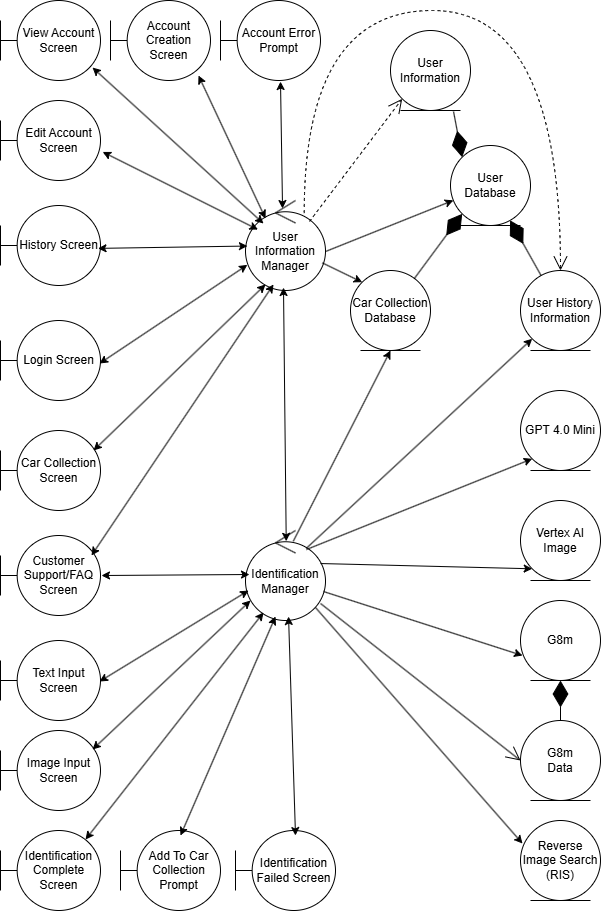
\includegraphics[scale=0.5]{images/AnalysisDiagram_compacted.png}\\
	\textbf{Figure 1.} Analysis class diagram for the RideRecon system, showing interactions between user interface screens, core system managers, databases, and expert modules for user management and vehicle identification.
\end{center}
% End Section


\section{Architectural Design}
\label{sec:architectural_design}
% Begin Section
This section should provide an overview of the overall architectural design of your application. Your overall architecture should show the division of the system into subsystems with high cohesion and low coupling.

\subsection{System Architecture}
\label{sub:system_architecture}
% Begin SubSection
The main architecture used in RideRecon is the Blackboard architecture. The Blackboard architecture style has several subsystems that are involved, as it utilizes the knowledge of up to four different agents, including Vertex AI Image, Google Reverse Image Search (RIS), text-based large-language model (LLM) and an internally trained machine learning (ML) program. These resources are These resources are integrated into the architecture through a Repository style so that each subsystem agent creates a hybrid architecture with both the Blackboard and Repository style.\\

\noindent The following subsystems that have been included in the architecture diagram have been defined below:\\

\noindent
\begin{tabular}{|p{4cm}|p{7cm}|p{3.5cm}|}
	\hline
	Subsystem & Purpose & Architectural Style \\
	\hline
	Account Management & Create, access, update, recover and authenticate account. & Repository \\
	\hline
	Collection Management & Create, view and edit a car collection. & Repository \\
	\hline
	Input Management & Identify a car through text or image and add to a collection afterwards (if desired). & Blackboard with each agent using Repository \\
	\hline
\end{tabular}

\\
\noindent Subsystem relationships and further explanation of their architecture are defined in Section 3.2 of this document.\\

\noindent In addition, there are three databases, each utilized by the different subsystems. The G8M stores all relevant information for the internally trained ML agent, present as an agent in the diagram as G8M. The account database and car collection database, respectively, store all account details and all relevant information required to create specific car collections.\\

\noindent As stated above, the architecture incorporates both Blackboard and Repository styles, with the overall architecture style being recognized as Blackboard. This is because the Blackboard architecture is recognized as the most significant for completing the main program functionality, which is car identification. The Blackboard style was chosen due to its ability to utilize many different domain-specific knowledge sources (i.e., the four different agents specified above) in order to collaborate together to solve a complex problem. In our case, the complex problem is being able to identify a car.\\

\noindent The nature of the Blackboard architecture is to be able to provide solutions to nondeterministic solutions, which is helpful for our program as we recognize that identification will always be bound by the limitations of the data covered by the specified agents. The ability of the Blackboard architecture to have different agents working in parallel allows our system to support identification through both image and text simultaneously, which is important for comprehensive identification. Additionally, using a Blackboard architecture style allows easy scalability through updating existing knowledge sources and adding new knowledge sources. This is beneficial to our system as we expect the expected app maintenance will require modifications to the knowledge sources in the event that their knowledge limitations are no longer acceptable.\\

\noindent The Repository architecture is also incorporated for  each knowledge sources in the Blackboard method as it allows multiple software component clients to access different aspects of large, complex information systems. In this case, the agents of the blackboard system are considered the clients that are requesting information needed to complete their partial solutions. This is beneficial for the system as it ensures that while agents work in parallel, they are able to access the relevant data stores that they need, even if another agent is currently accessing certain information from the data store. This also allows multiple users to operate the system at the same time, as the information system is able to be accessible to multiple instances of agents who are looking to identify different cars. Furthermore, if more agents are added to the Blackboard architecture, the Repository style ensures each new knowledge source will be able to easily access the necessary data store. The Repository style can also easily integrate additional protection measures, as it supports data integrity with an easy way to back up and restore information. Additionally, by also integrating the Repository style in Account and Collection Management subsystems, it ensures that the system is easily able to accommodate increases in new users in all aspects of app usage.\\

\begin{center}
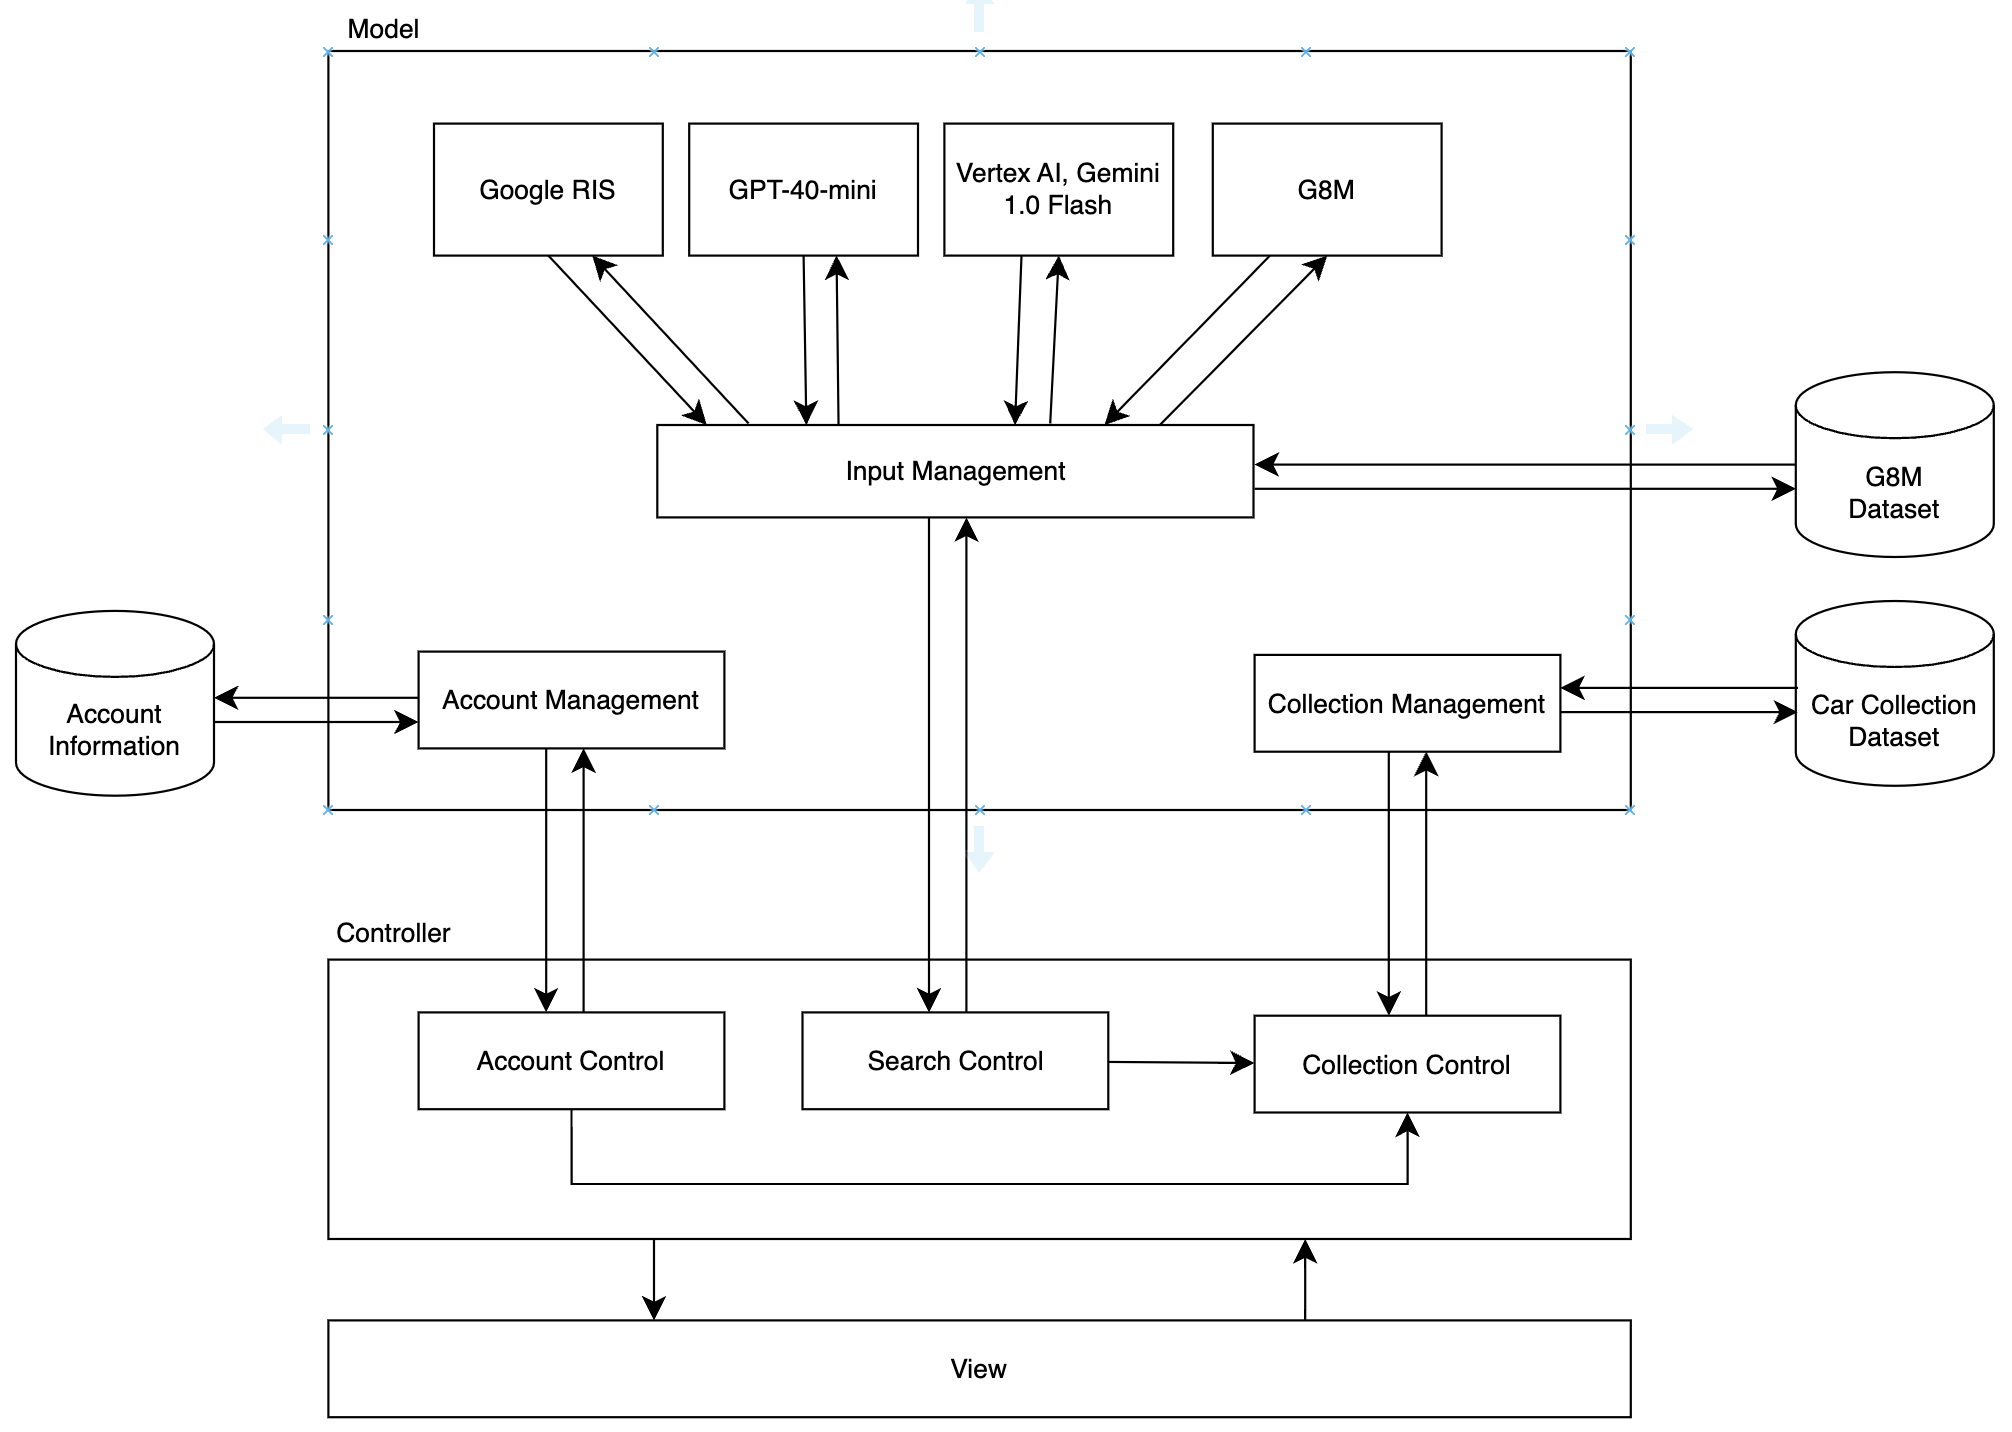
\includegraphics[scale=0.5]{images/system_architecture.png}
\textbf{Figure 2.} System Architecture.\\
\end{center}

\noindent \textbf{Why Batch Sequential architecture was not used:} Due to its rigid and sequential style of architecture, it lacks the real-time, iterative, and dynamic collaboration approach that is useful to solve complex problems such as identification. It also is unable to handle real-time updates due to its reliance on batched data sets, which is unsuitable as the system should be able to continuously adapt to new information in order to provide the best solution given all information provided.\\

\noindent \textbf{Why Pipe and Filter architecture was not used:} Similarly, to Batch Sequential architecture, the rigid nature of having specific defined processing steps in which it handles data makes it unsuitable for the dynamic collaboration required during an identification process.\\

\noindent \textbf{Why Process-Control architecture was not used:} This architecture is more rigid and better suited for a system with precise, well-defined target points in specific data that help determine fixed-logic decisions. Since identification involves uncertainty and dynamic reasoning, this makes it unideal for an architecture that relies on fixed rules and thresholds that shape the decision-making process.\\

% End SubSection

\subsection{Subsystems}
\label{sub:subsystems}
% Begin SubSection
The RideRecon system is divided into several key subsystems, each with a distinct role that contributes to the overall vehicle identification process. At its core, RideRecon employs a hybrid architecture that combines a blackboard approach—enabling multiple expert modules to collaboratively process inputs—with a repository-style design that robustly manages and stores data. This design not only ensures accurate vehicle identification but also supports continuous improvement through systematic data management.\\

\noindent The Input Management Subsystem is responsible for capturing and preprocessing user inputs, including both text and image data. It ensures that all input data is correctly formatted and validated before being fed into the core processing units. The Identification Subsystem acts as the central processing hub where diverse expert modules—such as the Vertex AI Image Model, Reverse Image Search, a specialized text-based LLM, and an internally trained ML model—post their analyses to a shared blackboard, collaboratively resolving any conflicts to produce a final identification. The Data Management Subsystem leverages repository principles to securely store both raw user inputs and processed outputs, which supports future retraining, auditing, and model improvement. Finally, the Account Management Subsystem handles user authentication and profile management, ensuring personalized interactions and maintaining a comprehensive record of user engagements. Together, these interconnected subsystems create a robust and scalable platform tailored to the challenges of dynamic, real-world vehicle identification.

% End SubSection

% End Section
	
\section{Class Responsibility Collaboration (CRC) Cards}
\label{sec:class_responsibility_collaboration_crc_cards}
% Begin Section
This section should contain all of your CRC cards.

\begin{itemize}
	\item Provide a CRC Card for each identified class
	\item Please use the format outlined in tutorial, i.e., 
	\begin{table}[ht]
		\centering
		\begin{tabular}{|p{5cm}|p{5cm}|}
		\hline 
		 \multicolumn{2}{|l|}{\textbf{Class Name:}} \\
		\hline
		\textbf{Responsibility:} & \textbf{Collaborators:} \\
		\hline
		\vspace{1in} & \\
		\hline
		\end{tabular}
	\end{table}
	
\end{itemize}
% End Section

\appendix
\section{Division of Labour}
\label{sec:division_of_labour}
% Begin Section
Include a Division of Labour sheet which indicates the contributions of each team member. This sheet must be signed by all team members.
% End Section
\begin{table}[h!]
\centering
\begin{tabular}{|p{3cm}|p{3.5cm}|p{3cm}|p{3cm}|p{3.5cm}|}
\hline
Hashim Bukhtiar & Jaden Moore & James Ariache & Olivia Reich & Omar Abdelhamid \\ \hline
1.1, 1.2, 3.2 & X Cards in Section 4 & Section 2 & Section 3.1 & Y Cards in Section 4 \\ 
Compiled Final Doc &  &  &  & Section 1.3 \\
\includegraphics[height=1cm]{../D1/images/hashim_signature.png} & \includegraphics[height=1cm]{../D1/images/Jaden_signature.jpg} &
\includegraphics[scale=0.1]{../D1/images/james_signature.png}& \includegraphics[height=0.6cm]{../D1/images/olivia_signature.png} & \includegraphics[height=0.6cm]{../D1/images/omar_signature.png}  \\
\hline
\end{tabular}
\caption{Division of Labour} 
\label{tab:division_of_labour}
\end{table}

\end{document}
%------------------------------------------------------------------------------